\documentclass[12pt,a4paper]{article}

% Encoding, Sprache, Schrift
\usepackage[ngerman]{babel}
\usepackage[T1]{fontenc}
\usepackage[utf8]{inputenc}
\usepackage{csquotes}
\renewcommand{\rmdefault}{ptm}

% Bilder einbinden
\usepackage{graphicx}
\graphicspath{ {picture/} }

% Seitenränder und sonstige Formate festlegen
\usepackage[a4paper,left=3cm,right=2cm,top=3cm,bottom=2.5cm]{geometry}
\usepackage{setspace}

%------------- Referenzen und Verzeichnisse -------------%
% Referenzen und URLs
\usepackage{url}
\usepackage{hyperref}
\usepackage{hyperxmp}
\hypersetup{
  colorlinks   = true,
  urlcolor     = black,
  linkcolor    = black,
  citecolor    = black
}
% Abbildungs + Tabellenverzeichnis
\usepackage[nottoc,numbib]{tocbibind}
% Listingverzeichnis
\usepackage{listings}
\renewcommand{\lstlistlistingname}{Listingverzeichnis}
% "Abb.", "Tbl." und "Lst."
\ifdefined\varShowTitlesInLists
  \makeatletter
  \renewcommand{\l@figure}[2]{\@dottedtocline{1}{1.5em}{2.3em}{Abb. #1}{#2}}
  \renewcommand{\l@table}[2]{\@dottedtocline{1}{1.5em}{2.3em}{Tbl. #1}{#2}}
  \renewcommand{\l@lstlisting}[2]{\@dottedtocline{1}{1.5em}{2.3em}{Lst. #1}{#2}}
  \makeatother
\fi
\newcommand{\varShowTitlesInLists}{true}
% Akronyme
\usepackage[acronym, nogroupskip, nonumberlist, nopostdot]{glossaries}
\loadglsentries{env/acronym.tex}
\makenoidxglossaries
\setacronymstyle{long-sc-short}
% Fußnoten
\usepackage[hang]{footmisc}
\renewcommand{\footnotemargin}{12pt}
% Unterschriften Bild + Tabelle
\usepackage[font=small, justification=centering]{caption}
% Literaturverzeichnis
\usepackage[style=ext-authoryear,     % ext- ermöglicht das Einblenden der Klammern um die Jahreszahl in Fußnoten
            sorting=nyt,              % Nach Nachnamen des ersten genannten Autorens sortieren, dann Jahr, dann Titel
            isbn=false,               % Ausblenden des Feldes
            url=false,                % Ausblenden des Feldes
            doi=true,                 % Einblenden des Feldes
            eprint=false,             % Ausblenden des Feldes
            clearlang=true,           % Ausblenden von Sprachcodes
            maxcitenames=2,           % Ab drei Autoren mit "et at." abkürzen
            citexref=true,            % Aufsplitten von Referenz in Sammelwerken
            mincrossrefs=0,           % Aufsplitten direkt bei der ersten Referenz auf Sammelwerk
            backref=true,             % Rückreferenzen vom Literaturverzeichnis in den Text
            maxbibnames=100]{biblatex}% Alle Autoren im Literaturverzeichnis ausschreiben
\addbibresource{content/references.bib}
\setcounter{biburllcpenalty}{1000}
% Ausblenden der Klammern um die Jahresangabe im Literaturverzeichnis
\ifdefined\varNoParenthesesAroundYear
  \makeatletter
  \def\act@on@bibmacro#1#2{%
    \expandafter#1\csname abx@macro@\detokenize{#2}\endcsname
  }
  \def\patchbibmacro{\act@on@bibmacro\patchcmd}
  \def\pretobibmacro{\act@on@bibmacro\pretocmd}
  \def\apptobibmacro{\act@on@bibmacro\apptocmd}
  \def\showbibmacro{\act@on@bibmacro\show}
  \makeatother

  \patchbibmacro{date+extradate}{%
  \printtext[parens]%
  }{%
  \setunit{\addperiod\space}%
  \printtext%
  }{}{}
\fi
%------------- Referenzen und Verzeichnisse -------------%

%--------------- Seitenspezifische imports --------------- %
% für Titelseite
\usepackage{chngpage}
\usepackage{calc}
\usepackage{float}
% Code
\usepackage{listings}
\usepackage{multicol}
\usepackage{wrapfig}
\usepackage{framed}
\usepackage[table]{xcolor}
%--------------- Seitenspezifische imports --------------- %


%-------------- sonstiges - nicht verwendet --------------%
% \usepackage{booktabs}
% \usepackage{enumitem}
% \usepackage[figure,table,lstlisting]{totalcount}

\title{Digitale Sichtung von Dokumenten zur Qualitätssicherung im Outputmanagement}
\author{Markus Schild}
\date{\today}

\newcommand{\varMartrikelnummer}{5007626}
\newcommand{\varArbeit}{Bachelorarbeit}
\newcommand{\varStudiengang}{Wirtschaftsinformatik}
\newcommand{\varUnternehmen}{mediserv Bank GmbH}
\newcommand{\varBetrBetreuer}{Peter Auer}
\newcommand{\varASWGutachter}{Prof. Dr. Dieter Hofbauer}
\newcommand{\varEingereichtAm}{27. Juli 2025}
%---------------------- Begriffe --------------------%
\newcommand{\mediserv}{mediserv Bank GmbH}
%---------------------- Begriffe --------------------%

%---------------------- Allgemein --------------------%
\newcommand{\asw}{ASW}

\newcommand{\vgl}[2]{\footcite[Vgl.][#2]{#1}}
\newcommand{\footrefnote}[2]{\footnote{Für das Thema #1 siehe Kapitel~\ref{#2}}}
\newcommand{\wholesection}[2]{\footcite[Für den gesamten Abschnitt vgl.][#2]{#1}}
%---------------------- Allgemein --------------------%

%-------------------- Sonstiges -----------------------%
% Wenn nach den 3 Ebenen nach \subsubsection eine weitere Gliederungsebene benötigt wird
\newcommand{\paragraphheader}[1]{\paragraph{#1}\mbox{}\\}

\newcommand{\varTitlepage}{env/titlepage.tex}
%-------------------- Sonstiges -----------------------%

\begin{document}

    \newgeometry{top=20mm,bottom=25mm}
\makeatletter
\begin{titlepage}
    \begin{figure}[t]
        \begin{adjustwidth}{-\oddsidemargin-1in}{-\rightmargin}

            \minipage{0pt}
              \noindent
              \makebox[0pt][l]{%
                \raisebox{-\totalheight}[0pt][0pt]{%
                  
\includegraphics[width=\paperwidth]{titlepage/banner_top}
                  }}%
            \endminipage

            \vspace*{10mm}
            \minipage{0.1\paperwidth}
              \hfill
            \endminipage
            \minipage{0.25\paperwidth}
              
\includegraphics[width=\linewidth]{titlepage/logo_asw.pdf}
            \endminipage
            \minipage{0.3\paperwidth}
                \hfill
            \endminipage
            \minipage{0.25\paperwidth}
              
\includegraphics[width=\linewidth]{logo_company.jpg}
            \endminipage

        \end{adjustwidth}
    \end{figure}

    \vspace*{2cm}

    \begin{flushleft}
        \Huge
        \textbf{\@title}\\[2cm]

        \LARGE
        {\@author}\\[0.5cm]

        \large
        Martrikelnummer: \varMartrikelnummer \\[0.5cm]

        \Large
        \varArbeit{} im Studiengang\\
        \varStudiengang
    \end{flushleft}

    \vspace{0.5cm}

    \begin{flushright}
        \ifdefvoid{\varBetrBetreuer}{}{%
            Betrieblicher Betreuer\\
            \varBetrBetreuer\\[0.5cm]
        }%

        ASW-Gutachter\\
        \varASWGutachter\\[0.5cm]

        Eingereicht am \varEingereichtAm
    \end{flushright}

    \begin{figure}[b]
        \begin{adjustwidth}{-\oddsidemargin-1in}{-\rightmargin}
            \noindent
            \makebox[0pt][l]{%
              \raisebox{-\totalheight}[0pt][0pt]{%
                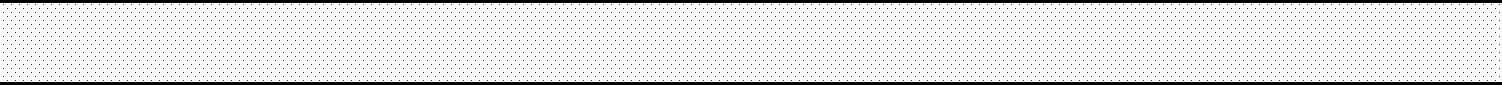
\includegraphics[width=\paperwidth]{titlepage/banner_bottom}}}%
        \end{adjustwidth}
    \end{figure}

\end{titlepage}
\makeatother
\restoregeometry

\newpage
    \newpage

    \pagenumbering{Roman}

    \setstretch{1.2}
\section*{Sperrvermerk}
Die vorliegende \varArbeit \space basiert auf internen, vertraulichen Daten und Informationen der \varUnternehmen.
In diese Arbeit dürfen Dritte, mit Ausnahme der Gutachter und befugten Mitgliedern des Prüfungsausschusses,
ohne ausdrückliche Zustimmung des Unternehmens und des Verfassers keine Einsicht nehmen. Eine Vervielfältigung
und Veröffentlichung der \varArbeit \space ohne ausdrückliche Genehmigung – auch auszugsweise – ist nicht erlaubt.
\setstretch{1}
\clearpage

    \tableofcontents
    \newpage

    \listoffigures
    \listoftables
    \addcontentsline{toc}{section}{Listingverzeichnis}
    \lstlistoflistings
    \newpage

    \addcontentsline{toc}{section}{Abkürzungsverzeichnis}
    \setstretch{0.5}
    \printnoidxglossary[type=acronym,sort=letter,style=listdotted,title=Abkürzungsverzeichnis]
    \newpage


    \setstretch{1.2}

\section{Einführung}
\subsection{Allgemein}
In der heutigen Zeit ist Umweltschutz ein wichtiges Thema
und auch schon kleine Änderungen können eine positive Wirkung haben.

Dabei ist die Arbeit mit Gesundheitsdaten, welche besondere personenbezogene Daten sind,
besonders schützenzwerte Informationen. % \vgl{eu_verordnung-dsgvo_2016}{Artikel 1, Artikel 4 \romannumeral{1} \romannumeral{15} }
\subsection{Motivation}
Durch eine größer werdende Anzahl an angekaufter Rechnungen erhöht sich gleichzeitig der Aufwand im Fachbereich.
Einige dieser Prozesse lassen sich dabei gut durch einen einheitlichen, digitalen Prozess abbilden,
der dabei nur mit geringen Systembrüchen einhergeht.

\subsection{Zielsetzung}
\subsection{Aufbau der Arbeit}


\acrfull{OPM}
\clearpage

    \printbibliography[heading=bibintoc]
    \clearpage

    \appendix
\clearpage

    \pagenumbering{gobble}
\section*{Persönliche Erklärung}

Hiermit erkläre ich, dass ich
\begin{enumerate}
  \item meine \varArbeit \space ohne fremde Hilfe angefertigt habe,
  \item die Übernahme wörtlicher Zitate aus der Literatur sowie die Verwendung von Gedanken anderer Autoren an den entsprechenden Stellen innerhalb der Arbeit gekennzeichnet habe und
  \item meine \varArbeit \space bei keiner anderen Prüfungsstelle vorgelegt habe.
\end{enumerate}
Ich bin mir bewusst, dass eine falsche Erklärung zum Nichtbestehen der \varArbeit \space führt.

\vspace{2cm}

\begin{tabular}{lp{2em}l}
 \hspace{5cm}   && \hspace{3cm} \\\cline{1-1}\cline{3-3}
 Ort, Datum     && Unterschrift
\end{tabular}


\end{document}
